\documentclass[conference]{IEEEtran}
\IEEEoverridecommandlockouts

\usepackage{cite}
\usepackage{amsmath,amssymb,amsfonts}
\usepackage{graphicx}
\usepackage{booktabs}
\usepackage{url}
\usepackage{hyperref}
\usepackage{multirow}
\usepackage{subcaption}
\hypersetup{colorlinks=true, linkcolor=black, citecolor=black, urlcolor=blue}

\graphicspath{{figures/}}

\begin{document}

\title{Open Mouth Is All You Need}

\author{
  \IEEEauthorblockN{Jaden Zhou}
  \IEEEauthorblockA{
    Khoury College of Computer Sciences\\
    Northeastern University\\
    zhou.jad@northeastern.edu
  }
}

\maketitle

% ── Abstract ──────────────────────────────────────────────────────────────────
\begin{abstract}
Automatically detecting when a speaker is talking in monocular video is useful
for lecture analytics, meeting summarization, and engagement monitoring.
Most existing approaches rely on audio or deep visual models, obscuring
which geometric cues actually drive performance.
We investigate which hand-crafted facial features are stable and informative
under natural appearance variation—lighting, head pose, and camera motion—using
a single-subject corpus of 30 lecture recordings.
A pipeline based on MediaPipe face landmarking extracts eight features per frame:
mouth openness, eye openness, head-pose yaw and pitch (via PnP), frame-difference
motion statistics, ambient brightness, and landmark detection confidence.
Logistic regression and SVM-RBF classifiers are trained on one recording and
evaluated on twenty held-out recordings without adaptation.
An ablation study reveals that mouth openness alone achieves F1\,=\,0.883,
matching the full eight-feature model (F1\,=\,0.881), while removing mouth
openness drops performance to F1\,=\,0.705.
Cross-video generalization across seventeen evaluable test recordings yields
F1\,=\,0.750--0.950 (mean 0.848); three recordings are excluded due to degenerate
class distributions or severe landmark occlusion and are analyzed separately.
Pose and motion condition analysis reveals variable sensitivity across sessions,
with larger frontal-vs.-angled gaps in recordings featuring extended head-down postures.
A fine-tuning experiment confirms that adding up to 100 labeled target-domain frames
provides no consistent improvement, further supporting the robustness of lip aperture
as a cross-domain feature.
\end{abstract}

\begin{IEEEkeywords}
speaking detection, facial landmarks, MediaPipe, head pose, appearance variation,
logistic regression, SVM
\end{IEEEkeywords}

% ── 1. Introduction ───────────────────────────────────────────────────────────
\section{Introduction}
\label{sec:intro}

Automated analysis of lecture and meeting recordings enables a range of downstream
applications: identifying active speakers for indexing, estimating engagement from
participation patterns, and generating structured transcripts aligned with visual
activity.
A fundamental sub-task is \emph{frame-level speaking detection}—determining, for
each video frame, whether the visible subject is currently producing speech.

Real-world recordings introduce appearance variation that can degrade feature
reliability.
Head pose changes as the speaker gestures or turns to write on a board.
Ambient lighting shifts between windows, projectors, and overhead sources.
Camera motion, zoom changes, and subject movement alter the pixel statistics of
every frame.
Prior work addressing talking and lip-movement detection has largely relied on
deep convolutional or recurrent architectures~\cite{chung2016out,chung2017lip},
which achieve high performance but provide little insight into which facial
geometry actually carries the signal.

We take a \emph{feature analysis} perspective: rather than maximizing accuracy
with a black-box model, we ask which hand-crafted geometric and photometric
features are individually informative, which are redundant, and how stable
each is under controlled appearance variation.
Our experimental design uses a strict video-level train/test split across
30 recordings of a single subject, enabling direct measurement of
cross-recording generalization without the confound of subject identity.

\textbf{Contributions.}
\begin{enumerate}
  \item An ablation study across nine feature subsets demonstrating that
        mouth openness is both necessary and sufficient for speaking detection
        at this task difficulty, with no measurable gain from adding pose,
        motion, or brightness features.
  \item A cross-video generalization study on twenty held-out recordings spanning
        the full semester, with condition-stratified evaluation (frontal vs.\ angled
        pose; low vs.\ high motion) identifying when and why performance degrades.
  \item A fine-tuning experiment showing that adding small labeled target-domain
        samples (25--100 frames) provides no consistent benefit, confirming that
        mouth openness generalizes without adaptation.
  \item A fully reproducible CPU-only pipeline using MediaPipe~\cite{kartynnik2019realtime}
        and scikit-learn, with annotated ground truth and released code.
\end{enumerate}

% ── 2. Related Work ───────────────────────────────────────────────────────────
\section{Related Work}
\label{sec:related}

\textbf{Lip reading and talking-face detection.}
Chung and Zisserman~\cite{chung2016out} trained a CNN on lip crops to synchronize
audio and video, demonstrating that visual lip motion provides strong signal for
speech activity.
Chung et al.~\cite{chung2017lip} extended this to sentence-level lip reading
from frontal video, showing that deep networks can extract rich articulatory
features—but requiring large annotated corpora and GPU-scale training.
Our work differs by studying \emph{which} geometric features drive performance
in a resource-constrained, single-subject setting rather than maximizing accuracy
with deep models.

\textbf{Active speaker detection.}
Roth et al.~\cite{roth2020ava} released the AVA-ActiveSpeaker dataset and
benchmarked audio-visual models for detecting which face in a multi-speaker scene
is talking.
Their best systems fuse audio with visual lip features, underscoring the primacy
of mouth region information—consistent with our ablation finding that mouth
openness dominates.
We focus on the visual-only case with a single subject, isolating feature
geometry from audio and multi-face disambiguation.

\textbf{Head pose estimation.}
Ruiz et al.~\cite{ruiz2018finegrained} proposed a CNN-based head-pose estimator
trained on synthetically augmented data, achieving fine-grained yaw/pitch/roll
without landmark supervision.
We adopt the classical PnP approach using MediaPipe landmarks as a lightweight,
interpretable alternative suitable for CPU-only deployment.
Our generalization results confirm that pose variation up to the range present
in lecture recordings does not significantly degrade mouth-openness-based
speaking detection.

\textbf{Face landmarking.}
Kartynnik et al.~\cite{kartynnik2019realtime} introduced the MediaPipe Face
Mesh model, producing 468 3D landmarks in real time on mobile hardware.
We use this model as our feature extraction backbone, leveraging its landmark
indices for mouth, eye, and pose computation.

% ── 3. Methods ────────────────────────────────────────────────────────────────
\section{Methods}
\label{sec:methods}

\subsection{Dataset and Annotation}

Our corpus consists of 30 lecture recordings of a single subject captured with
a fixed webcam at standard definition.
One recording (video \texttt{20260107-1}, approximately 45 minutes) serves as the
training split; all twenty remaining recordings spanning the full semester serve
as the test split.
Frames are extracted at a 10-frame interval (approximately 3 fps from a 30 fps
source), yielding 1,179 labeled training frames and 5,656 labeled test frames
across the twenty test videos.
Two test recordings (\texttt{20260107-2}, \texttt{20260108-2}) have zero or
near-zero speaking instances and are excluded from aggregate metrics;
one recording (\texttt{20260219}) is flagged as an outlier due to extended
head-down posture (see Section~\ref{sec:discussion}).

Ground-truth labels are binary: \textit{speaking} (1) or \textit{silent} (0).
Labeling criterion is lip tension and movement continuity rather than
instantaneous mouth aperture to avoid a circular dependency with the primary
feature.
Ambiguous frames (laughing, occluded face, mid-intake breath) are excluded
from evaluation.

\begin{figure}[t]
  \centering
  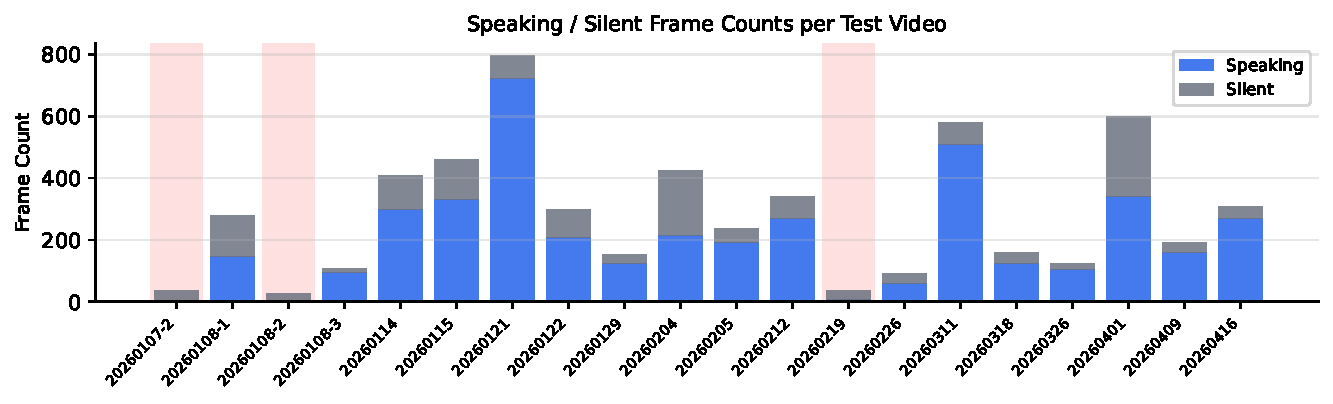
\includegraphics[width=\columnwidth]{class_balance.pdf}
  \caption{Speaking and silent frame counts per test video (sorted chronologically).
           Red-shaded bars mark the three sessions excluded from aggregate statistics:
           \texttt{20260107-2} (2 speaking frames),
           \texttt{20260108-2} (0 speaking frames), and
           \texttt{20260219} (mouth frequently occluded).}
  \label{fig:class_balance}
\end{figure}

\begin{figure}[t]
  \centering
  \begin{subfigure}[b]{0.48\columnwidth}
    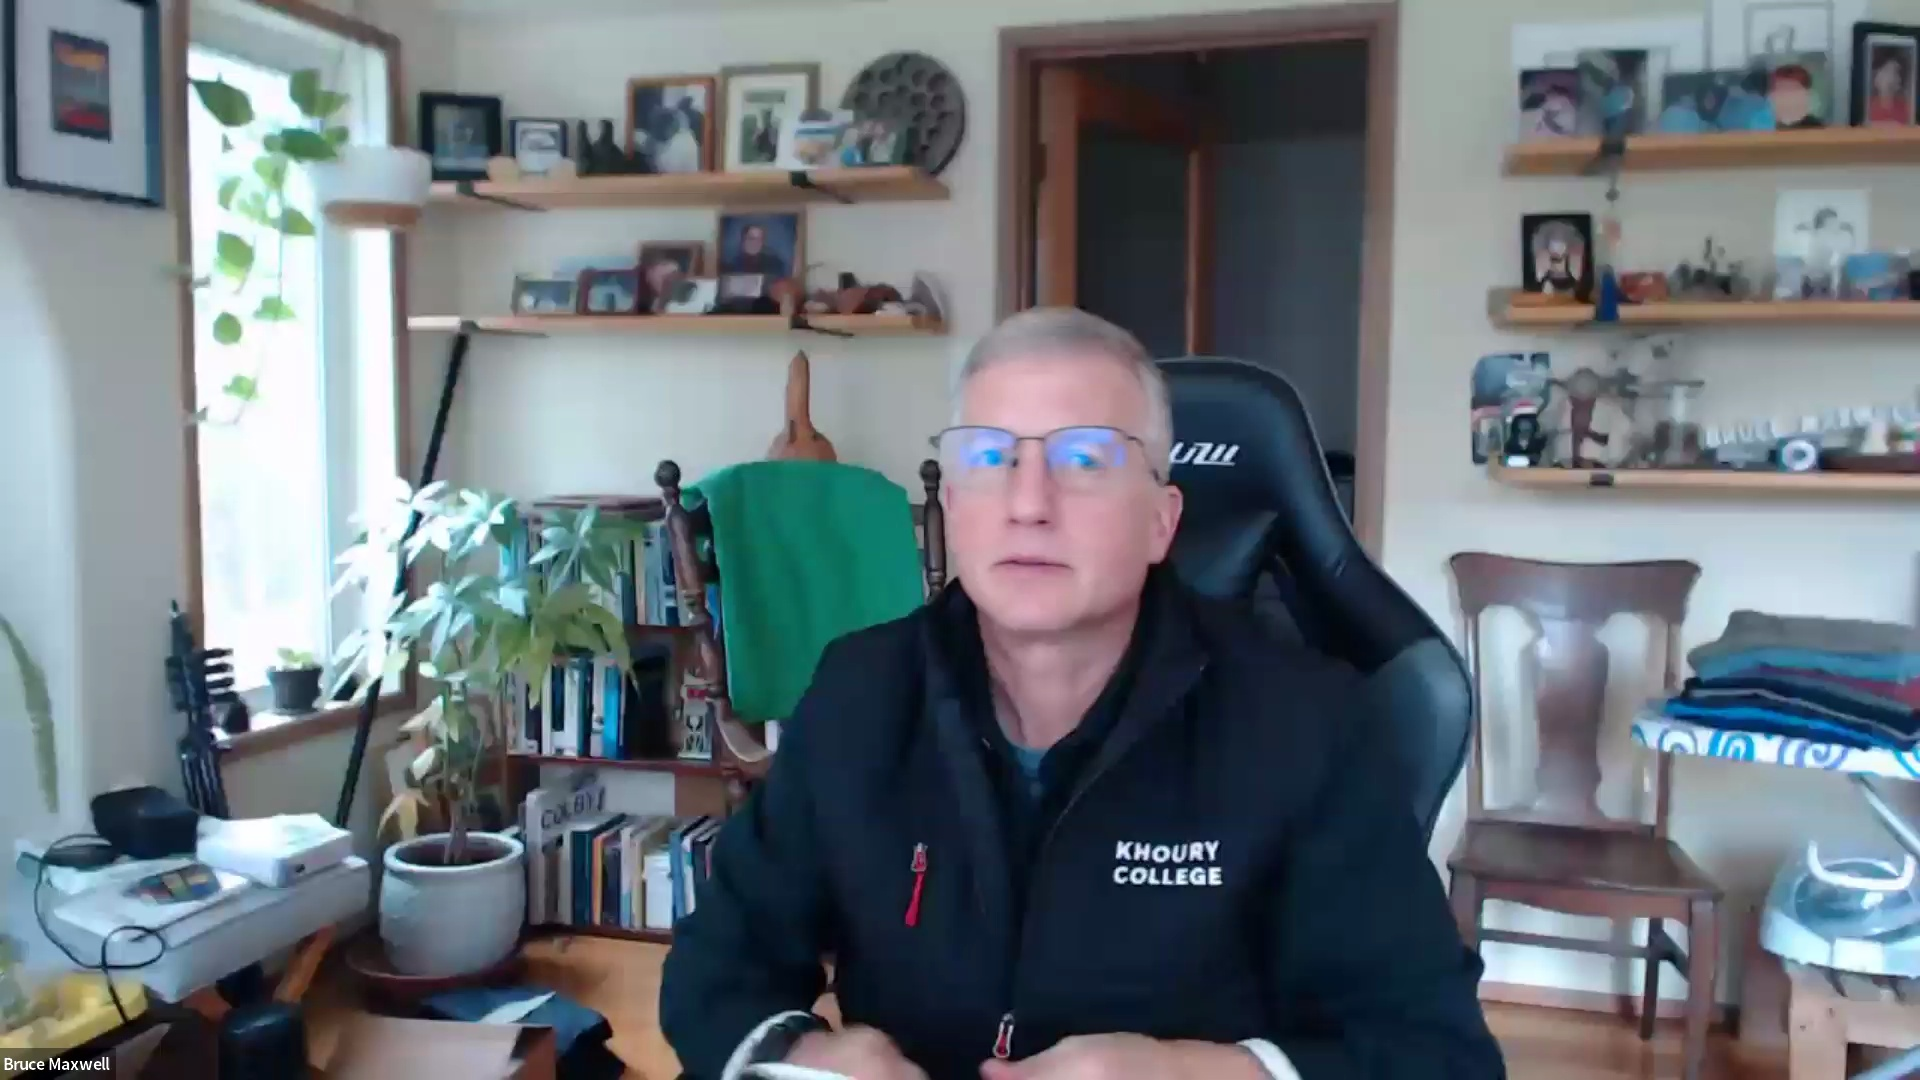
\includegraphics[width=\linewidth]{0000110.jpg}
    \caption{Frontal, silent (baseline)}
    \label{fig:frame_baseline}
  \end{subfigure}
  \hfill
  \begin{subfigure}[b]{0.48\columnwidth}
    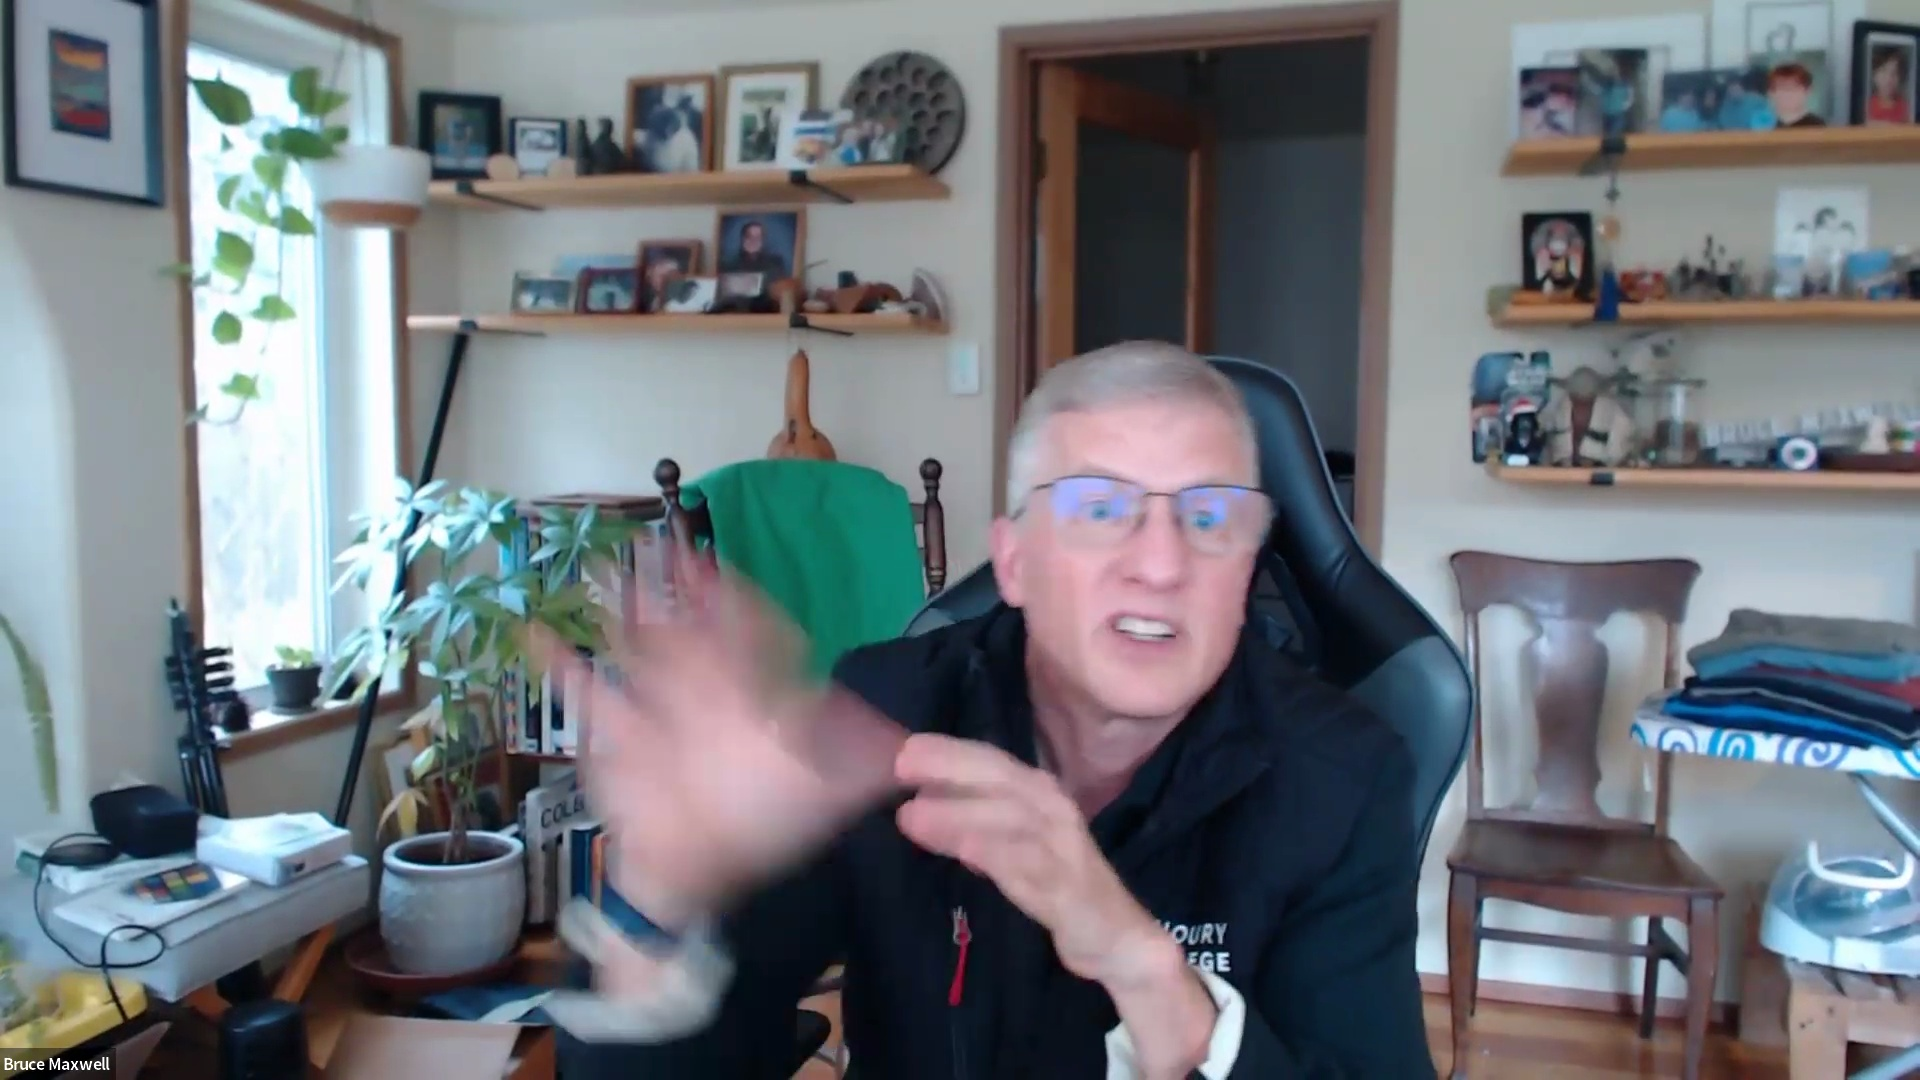
\includegraphics[width=\linewidth]{0014750.jpg}
    \caption{Speaking with hand gesture}
    \label{fig:frame_speaking}
  \end{subfigure}

  \vspace{4pt}

  \begin{subfigure}[b]{0.48\columnwidth}
    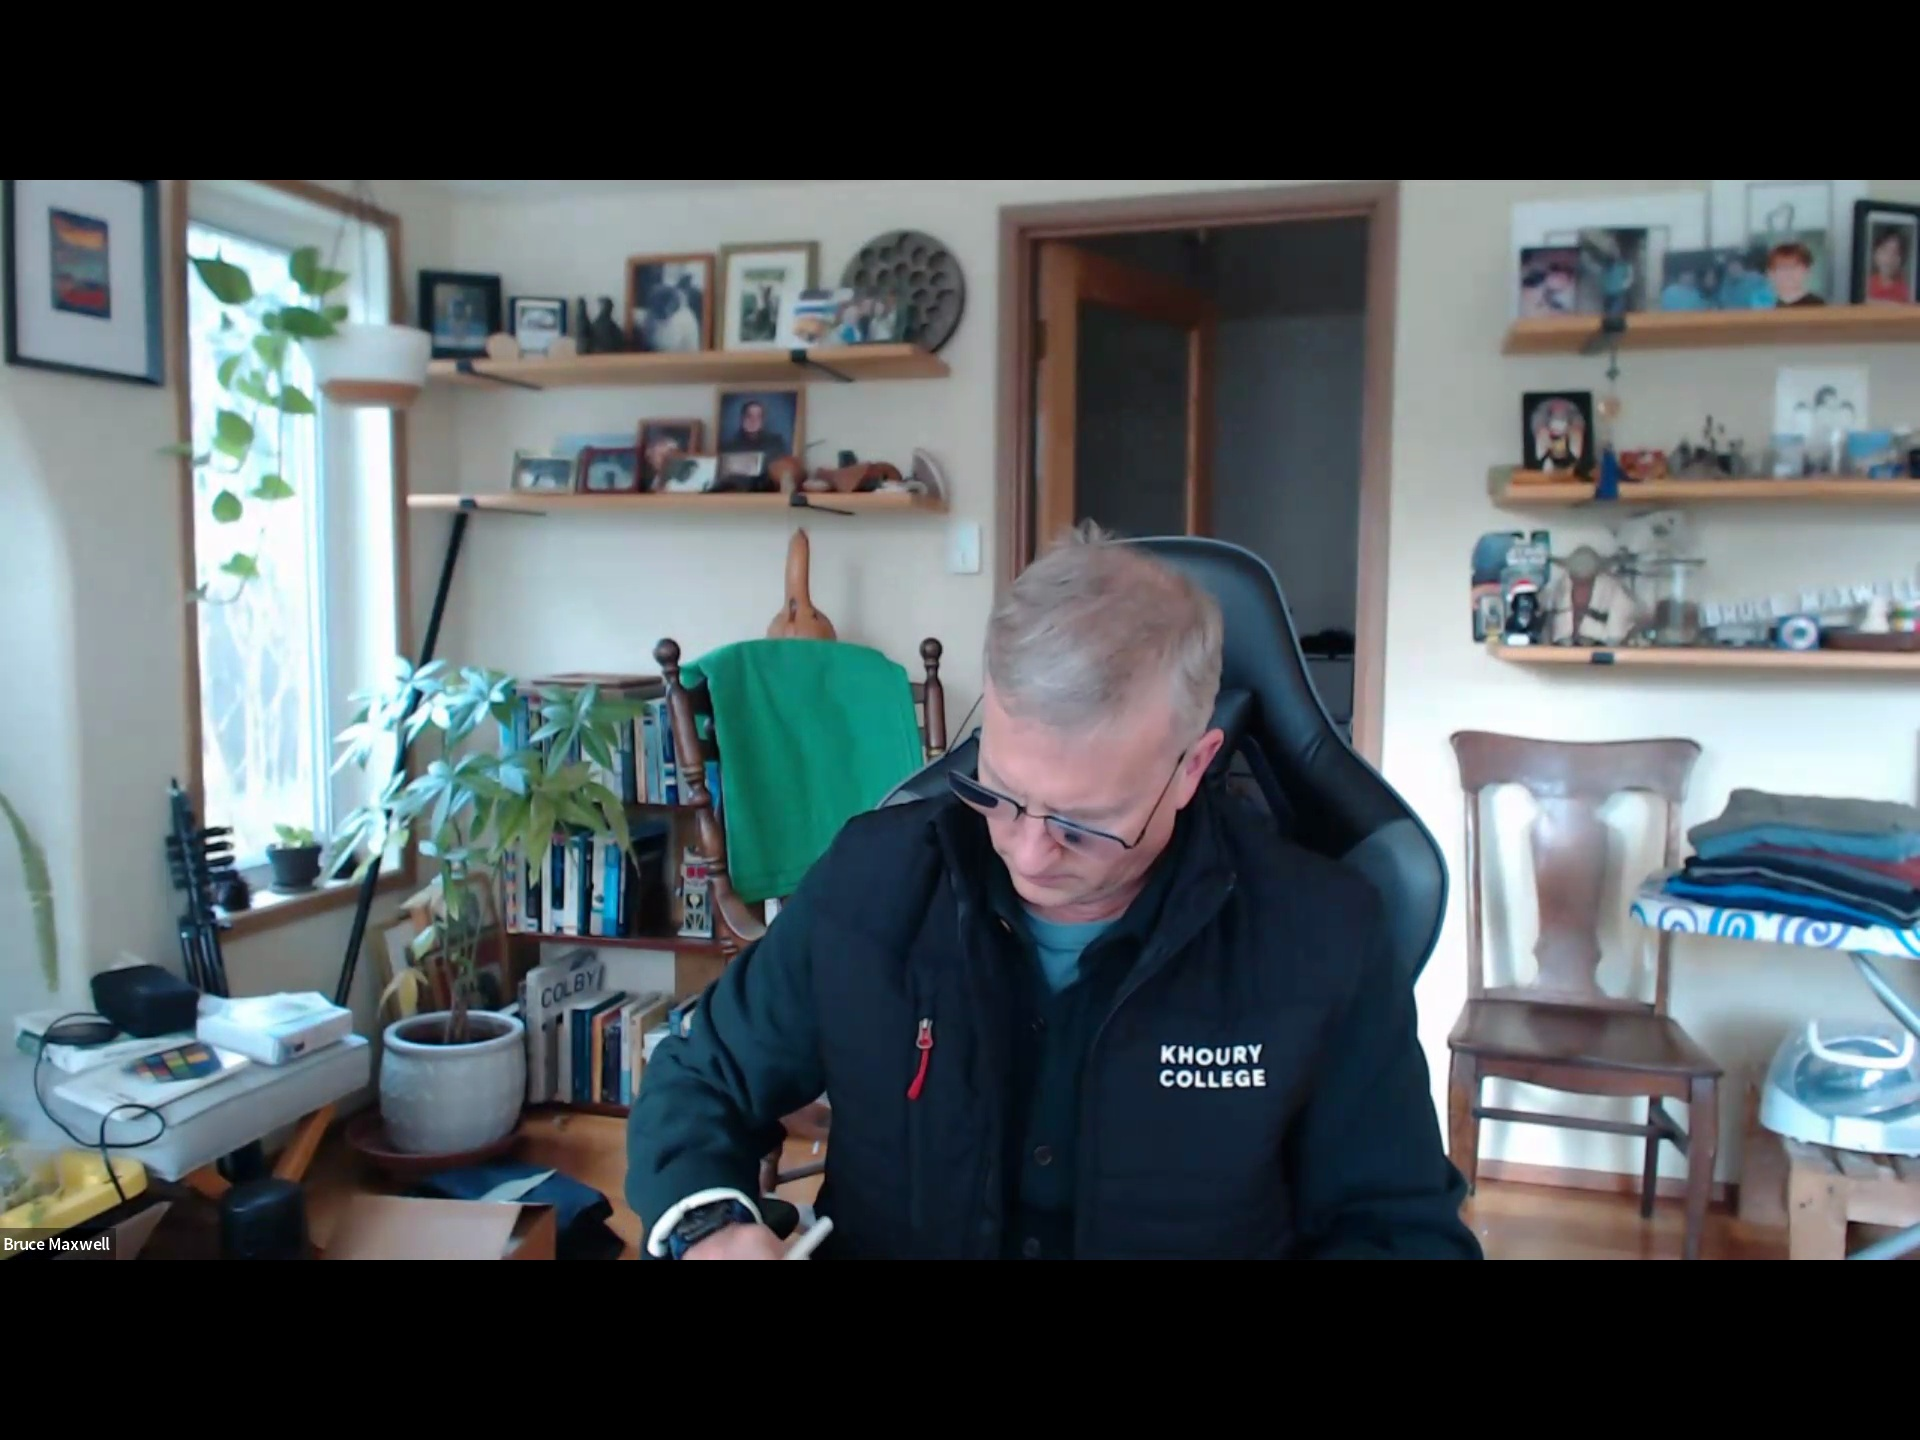
\includegraphics[width=\linewidth]{0000890.jpg}
    \caption{Head-down posture (mouth occluded)}
    \label{fig:frame_headdown}
  \end{subfigure}
  \hfill
  \begin{subfigure}[b]{0.48\columnwidth}
    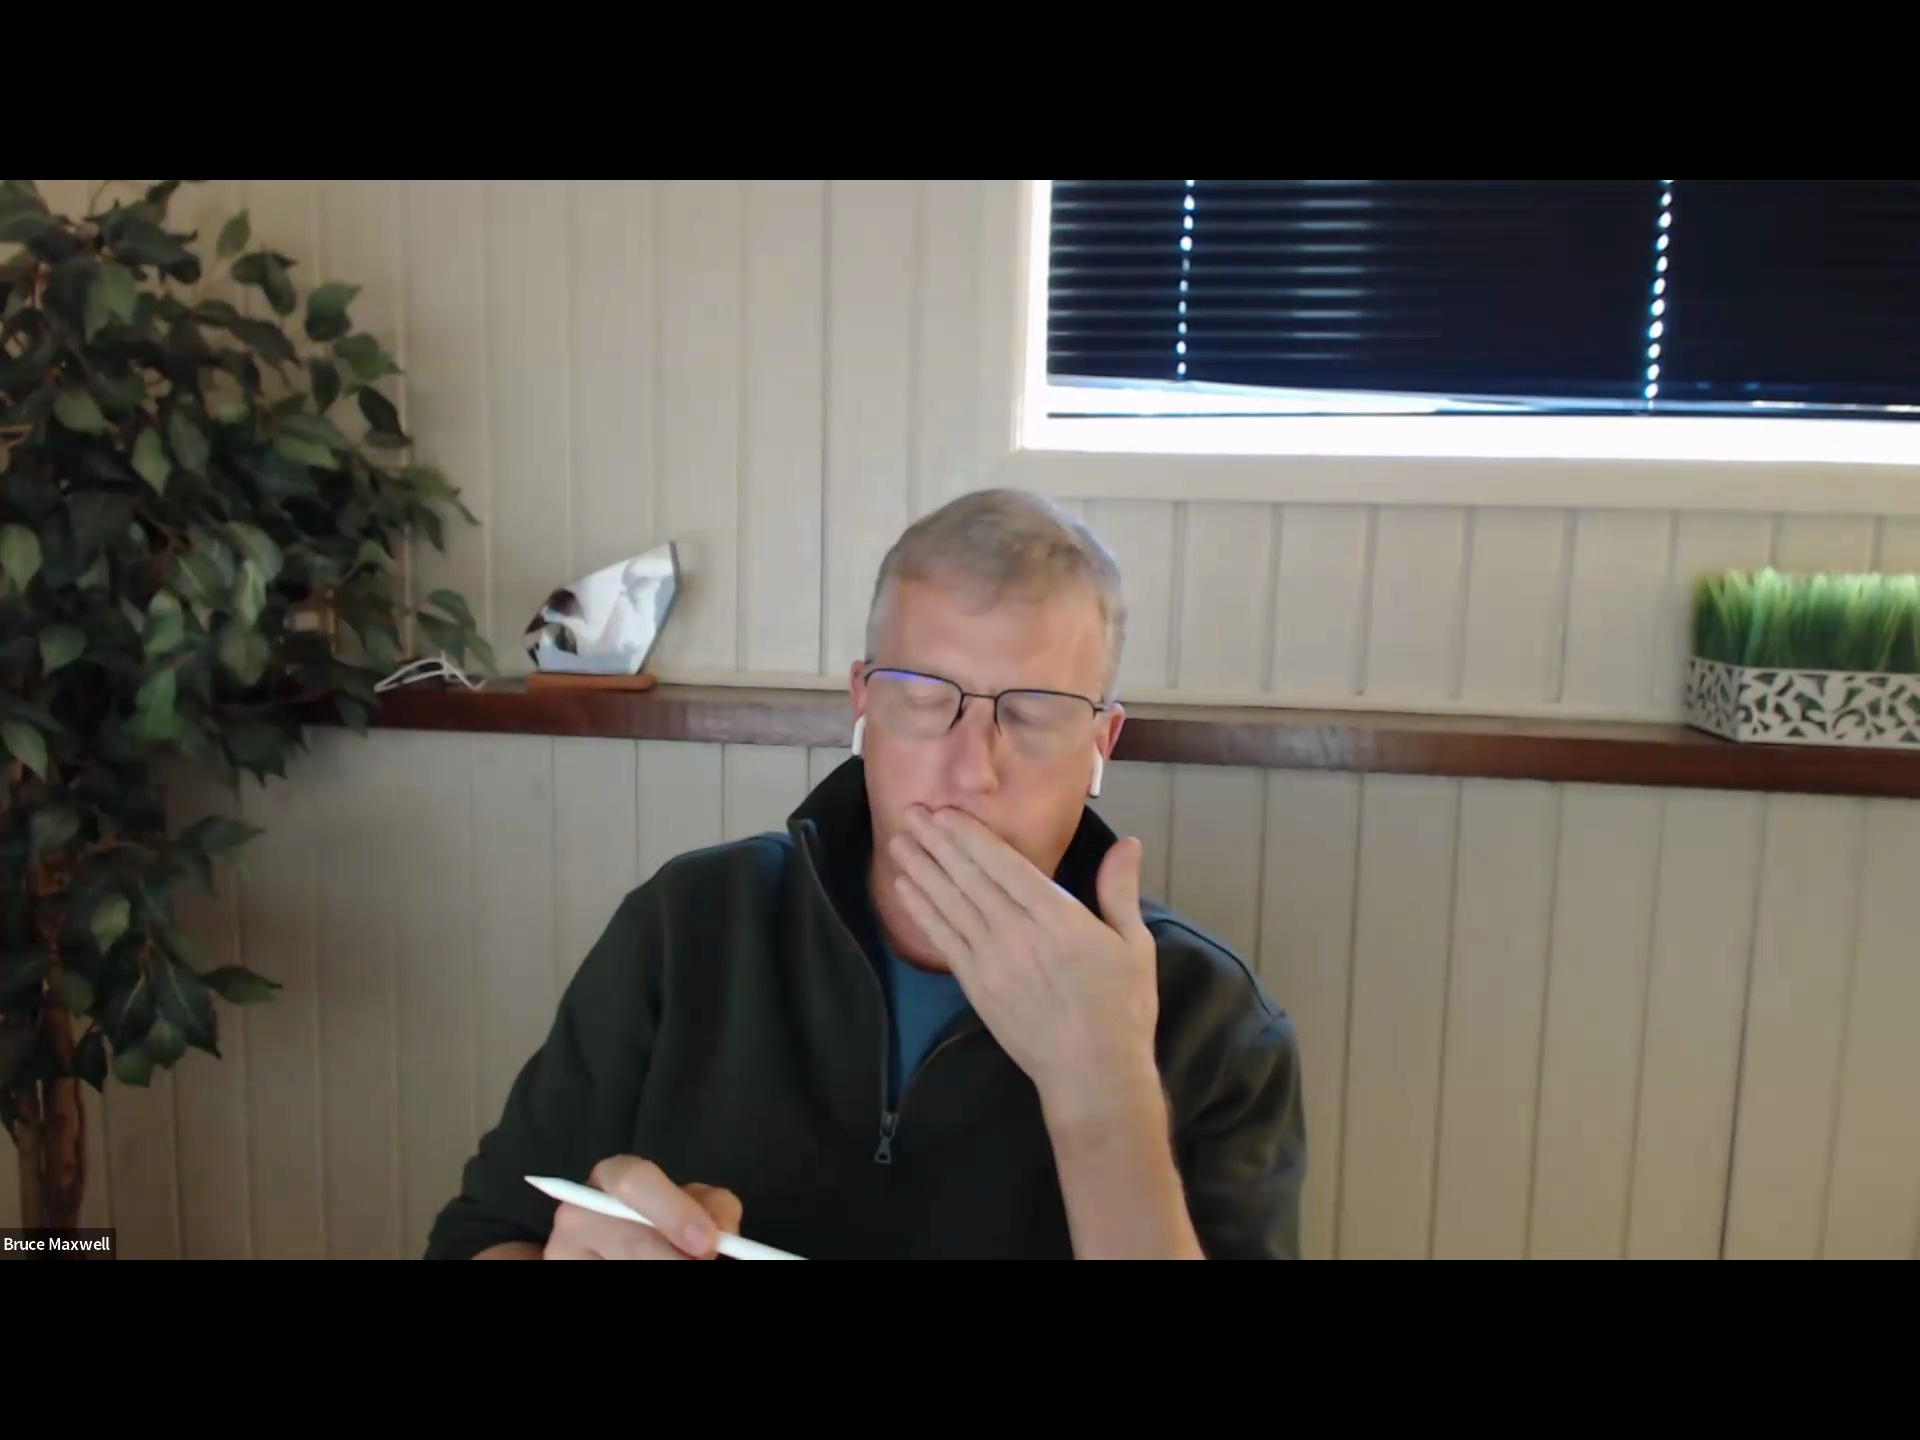
\includegraphics[width=\linewidth]{0000160.jpg}
    \caption{Hand covering mouth (occlusion)}
    \label{fig:frame_occlusion}
  \end{subfigure}

  \caption{Representative frames illustrating appearance variation in the corpus.
           (a) Clean frontal baseline. (b) Active speech with gestural motion blur.
           (c) Head-down writing posture—the primary failure mode in
               \texttt{20260219}, where the mouth exits the camera's field of view.
           (d) Hand occlusion of the mouth region, a confound for landmark-based
               mouth openness.}
  \label{fig:example_frames}
\end{figure}

\subsection{Feature Extraction}

We extract eight features per frame using MediaPipe Face Landmarker
(468 3D landmarks, minimum detection confidence 0.5):

\begin{itemize}
  \item \textbf{Mouth openness}: Euclidean distance between landmarks \#13
        (upper inner lip) and \#14 (lower inner lip), scaled by frame height.
        A higher value indicates a more open mouth.

  \item \textbf{Eye openness}: Average of left and right eyelid spans
        (landmarks \#386/374 and \#159/145 respectively), same normalization.

  \item \textbf{Yaw and pitch}: Head pose estimated via the Perspective-n-Point
        (PnP) algorithm~\cite{opencv} using six landmark-to-3D correspondences
        (nose tip, chin, eye corners, mouth corners).
        Yaw encodes left-right rotation; pitch encodes up-down tilt, both in degrees.

  \item \textbf{motion\_mean, motion\_var}: Mean and variance of pixel-wise absolute
        frame differences between consecutive grayscale frames, measuring camera
        and subject motion.

  \item \textbf{Brightness}: Mean grayscale intensity of the full frame (0--255),
        as a proxy for ambient lighting.

  \item \textbf{Landmark confidence}: Binary indicator (1.0 if landmarks detected,
        0.0 otherwise).
\end{itemize}

Frames with missing landmark detections receive \texttt{NaN} for landmark-dependent
features; such frames are excluded from all analyses via \texttt{dropna}.

\subsection{Variation Conditions}

To enable condition-stratified analysis, frames are assigned discrete appearance
conditions using thresholds calibrated on the training distribution:

\begin{itemize}
  \item \textbf{Pose}: frontal ($|\text{yaw}| < 15^\circ$)
        vs.\ angled ($|\text{yaw}| \geq 15^\circ$).
        The $15^\circ$ boundary is standard in the pose literature and
        splits the training data approximately 38/62 frontal/angled.

  \item \textbf{Lighting}: high (brightness $> 115$)
        vs.\ low ($\leq 115$, the 25th percentile of training brightness).

  \item \textbf{Motion}: low (motion\_mean $< 5.3$)
        vs.\ high ($\geq 5.3$, the training median, giving a near 50/50 split).
\end{itemize}

Absolute thresholds (rather than per-video relative thresholds) are used so that
condition labels carry consistent real-world meaning across all test recordings.

\subsection{Classifiers}

Both classifiers operate on $z$-score normalized features
(StandardScaler fit on training data only):

\begin{itemize}
  \item \textbf{Logistic Regression} (L2 regularization, $C\!=\!1$,
        \texttt{max\_iter}=1000, \texttt{class\_weight=balanced}).
  \item \textbf{SVM-RBF} (RBF kernel, \texttt{class\_weight=balanced}).
\end{itemize}

Balanced class weighting compensates for the moderate speaking/silent imbalance
present in several test recordings.
Both models are trained once on all non-NaN training frames and applied without
adaptation to each test video.

\subsection{Evaluation Protocol}

\textbf{Experiment 1 (Ablation)} uses five-fold stratified cross-validation on the
training video to estimate within-distribution feature importance across nine feature
subsets (Table~\ref{tab:ablation}, Fig.~\ref{fig:ablation}).
The primary metric is F1 score (harmonic mean of precision and recall), which is
more informative than accuracy under class imbalance.

\textbf{Experiment 2 (Generalization)} evaluates the frozen model trained on
\texttt{20260107-1} on each of the twenty test videos independently.
Per-video F1, accuracy, and pose-condition (frontal vs.\ angled) F1 are reported
(Table~\ref{tab:generalization}, Fig.~\ref{fig:generalization}).

\textbf{Experiment 3 (Fine-tuning)} tests whether augmenting the training set with
a small stratified sample of labeled frames from the target video recovers
performance. Evaluated on five representative test videos with
$n \in \{25, 50, 100\}$ added frames (Table~\ref{tab:finetuning}).

% ── 4. Experiments and Results ────────────────────────────────────────────────
\section{Experiments and Results}
\label{sec:results}

\subsection{Experiment 1: Ablation Study}

Fig.~\ref{fig:feature_dist} shows the distribution of five features split by
speaking/silent label on the training video.
Mouth openness is the only feature with a clear separation between classes;
the remaining features have substantially overlapping distributions, foreshadowing
the ablation results.

\begin{figure}[t]
  \centering
  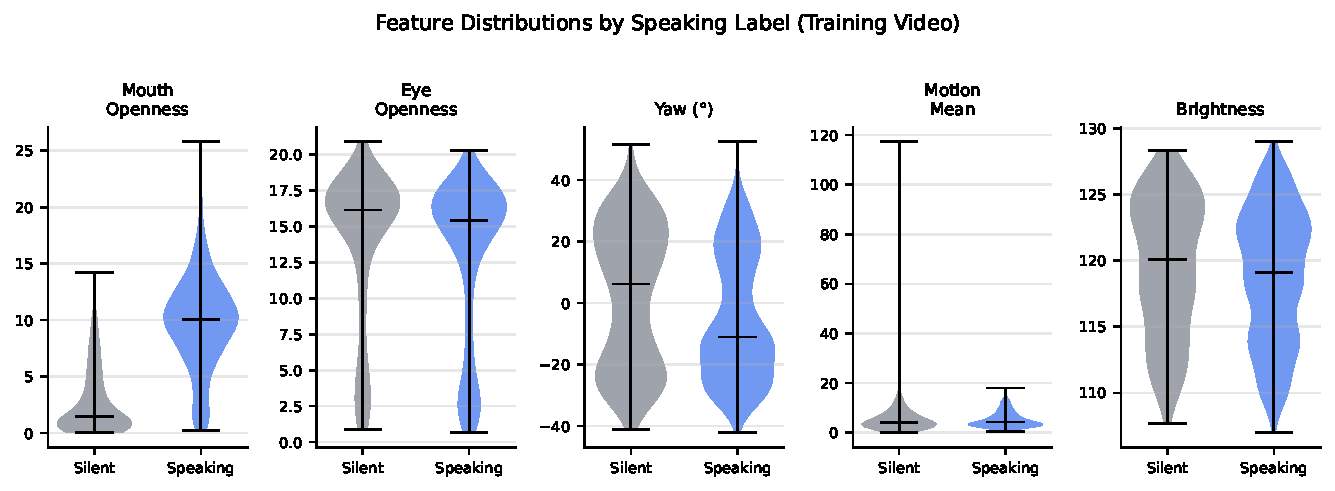
\includegraphics[width=\columnwidth]{feature_dist.pdf}
  \caption{Feature distributions by speaking label on the training video
           (violin plots; horizontal line = median).
           Mouth openness shows the clearest class separation.
           The remaining features have substantially overlapping distributions.}
  \label{fig:feature_dist}
\end{figure}

Table~\ref{tab:ablation} and Fig.~\ref{fig:ablation} report mean F1 ($\pm$1 std)
from five-fold cross-validation on the training video for nine feature subsets
and two classifiers.

\begin{table}[t]
\caption{Ablation Study — 5-fold CV F1 on Training Video}
\label{tab:ablation}
\centering
\setlength{\tabcolsep}{4pt}
\begin{tabular}{lcc}
\toprule
\textbf{Feature Subset} & \textbf{LogReg F1} & \textbf{SVM-RBF F1} \\
\midrule
Eye only           & 0.444 $\pm$ 0.029 & 0.605 $\pm$ 0.031 \\
Motion only        & 0.488 $\pm$ 0.023 & 0.693 $\pm$ 0.026 \\
Brightness only    & 0.587 $\pm$ 0.028 & 0.746 $\pm$ 0.010 \\
No mouth (7 feat.) & 0.705 $\pm$ 0.030 & 0.697 $\pm$ 0.060 \\
Pose only          & 0.717 $\pm$ 0.026 & 0.730 $\pm$ 0.051 \\
All features (8)   & 0.881 $\pm$ 0.009 & 0.885 $\pm$ 0.012 \\
No motion (6 feat.)& 0.883 $\pm$ 0.008 & 0.883 $\pm$ 0.012 \\
\textbf{Mouth only}& \textbf{0.883 $\pm$ 0.009} & \textbf{0.879 $\pm$ 0.012} \\
No pose (6 feat.)  & 0.885 $\pm$ 0.003 & 0.880 $\pm$ 0.011 \\
\bottomrule
\end{tabular}
\end{table}

\begin{figure}[t]
  \centering
  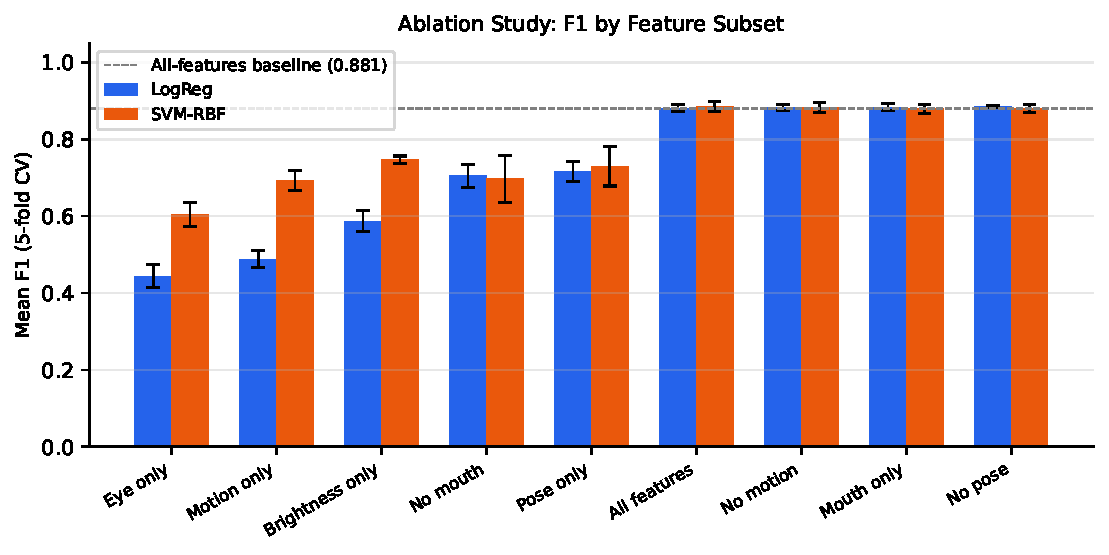
\includegraphics[width=\columnwidth]{ablation.pdf}
  \caption{Ablation study F1 by feature subset (5-fold CV, training video).
           Error bars show $\pm$1 standard deviation.
           Dashed line marks the all-features LogReg baseline (0.881).}
  \label{fig:ablation}
\end{figure}

The results reveal a clear bimodal structure.
Individual features—eye openness (0.444), motion (0.488), brightness (0.587),
and pose (0.717)—all fall well below the mouth-containing configurations.
Notably, SVM-RBF narrows the gap for some single features (e.g., brightness
0.746, motion 0.693), suggesting that nonlinear boundaries capture weak signal;
logistic regression does not.
Any combination retaining mouth openness performs comparably: removing motion
(0.883), removing pose (0.885), or using all eight features (0.881) all yield
F1 statistically indistinguishable from mouth openness alone (0.883).
Critically, removing mouth openness while retaining all seven other features
drops LogReg F1 to 0.705—an 18-point absolute decrease.

\textbf{Finding 1}: Mouth openness is both necessary and sufficient for
speaking detection in this corpus.
No other single feature approaches its predictive power, and no combination
of other features recovers comparable performance.

\subsection{Experiment 2: Cross-Video Generalization}

\begin{table}[t]
\caption{Generalization — LogReg on All Twenty Test Recordings.
         $\Delta_p$ = $|$frontal F1 $-$ angled F1$|$.
         Mean row excludes the three marked recordings.}
\label{tab:generalization}
\centering
\footnotesize
\setlength{\tabcolsep}{3pt}
\begin{tabular}{lccccc}
\toprule
\textbf{Video} & \textbf{F1} & \textbf{Acc} &
\textbf{Frontal} & \textbf{Angled} & \textbf{$\Delta_p$} \\
\midrule
20260107-2$^\dagger$ & 0.400 & 0.833 & 0.667 & 0.286 & 0.381 \\
20260108-1 & 0.826 & 0.782 & 0.806 & 0.837 & 0.031 \\
20260108-2$^\ddagger$ & 0.000 & 0.115 & --- & --- & --- \\
20260108-3 & 0.945 & 0.896 & 0.936 & 0.967 & 0.031 \\
20260114   & 0.950 & 0.924 & 0.956 & 0.929 & 0.027 \\
20260115   & 0.793 & 0.683 & 0.819 & 0.672 & 0.147 \\
20260121   & 0.941 & 0.895 & 0.928 & 0.946 & 0.018 \\
20260122   & 0.899 & 0.846 & 0.874 & 0.909 & 0.035 \\
20260129   & 0.863 & 0.773 & 0.937 & 0.791 & 0.146 \\
20260204   & 0.912 & 0.906 & 0.897 & 0.916 & 0.019 \\
20260205   & 0.770 & 0.674 & 0.787 & 0.698 & 0.089 \\
20260212   & 0.752 & 0.664 & 0.743 & 0.761 & 0.018 \\
20260219$^*$  & 0.316 & 0.639 & 0.667 & 0.250 & 0.417 \\
20260226   & 0.842 & 0.800 & 0.902 & 0.794 & 0.108 \\
20260311   & 0.798 & 0.691 & 0.875 & 0.765 & 0.110 \\
20260318   & 0.816 & 0.734 & 0.879 & 0.760 & 0.119 \\
20260326   & 0.750 & 0.645 & 0.872 & 0.610 & 0.262 \\
20260401   & 0.880 & 0.848 & 0.880 & 0.880 & 0.000 \\
20260409   & 0.777 & 0.674 & 0.753 & 0.789 & 0.036 \\
20260416   & 0.893 & 0.828 & 0.919 & 0.861 & 0.058 \\
\midrule
\textbf{Mean (17)} & \textbf{0.848} & \textbf{0.780} & 0.869 & 0.817 & 0.074 \\
\bottomrule
\end{tabular}
\vspace{2pt}

{\footnotesize
$^\dagger$2 speaking instances; F1 unreliable, excluded from mean.\\
$^\ddagger$27 total frames, 0 speaking; excluded from mean.\\
$^*$Extended head-down posture; mouth frequently occluded (see Sec.~\ref{sec:discussion}).}
\end{table}

\begin{figure}[t]
  \centering
  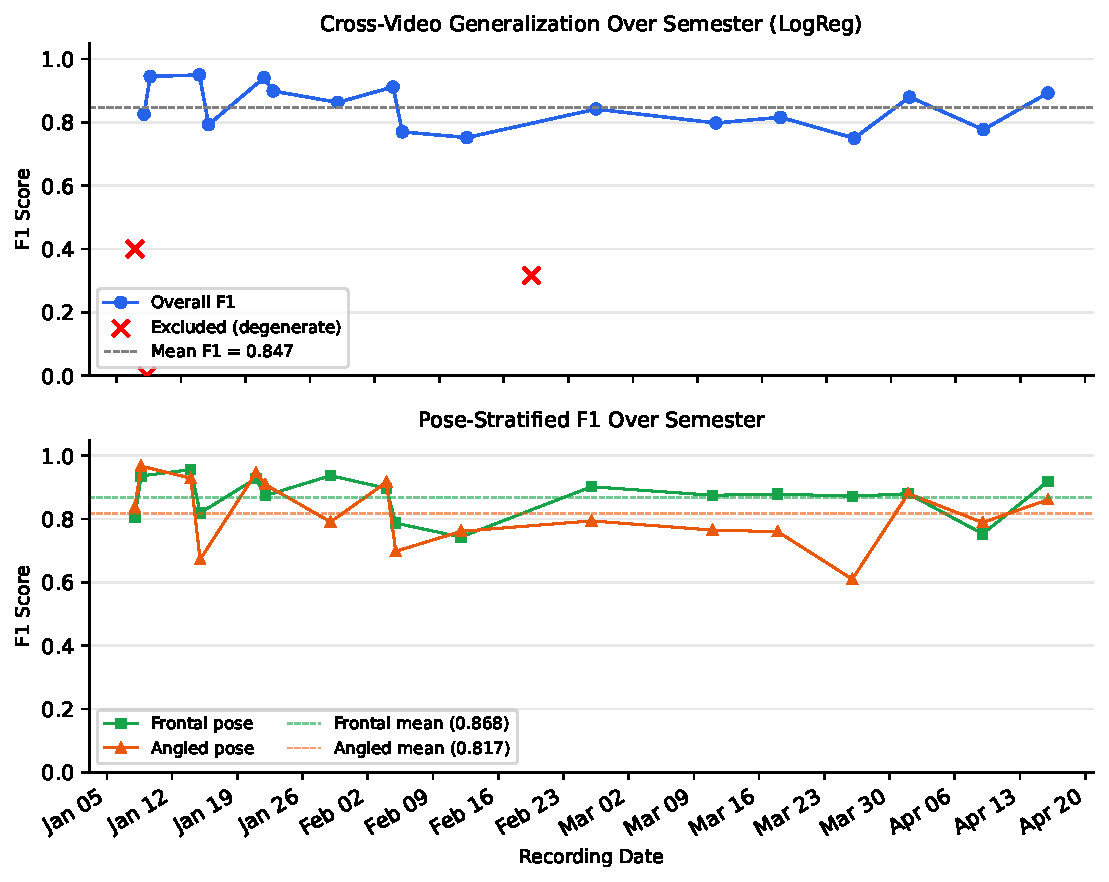
\includegraphics[width=\columnwidth]{generalization.pdf}
  \caption{Cross-video generalization over the semester (LogReg, all-features model).
           \emph{Top}: overall F1 per recording; red crosses mark sessions excluded
           from aggregate statistics. Dashed line shows mean F1\,=\,0.848 over
           17 valid recordings.
           \emph{Bottom}: frontal vs.\ angled pose F1 over time
           (means 0.869 and 0.817, respectively).}
  \label{fig:generalization}
\end{figure}

Table~\ref{tab:generalization} and Fig.~\ref{fig:generalization} show per-video
results across all twenty test recordings.
The model, trained on a single 45-minute recording, achieves F1\,=\,0.750--0.950
(mean 0.848) on the 17 evaluable recordings without any adaptation.

\textbf{Pose sensitivity.}
The frontal vs.\ angled F1 gap ($\Delta_p$) averages 0.074 across valid videos,
with a wide range (0.000--0.262).
Ten of seventeen videos show frontal F1 exceeding angled F1, consistent with
some degradation at larger yaw angles.
However, several videos show the opposite (e.g., \texttt{20260108-1},
\texttt{20260121}, \texttt{20260122}), suggesting that session-specific
correlations between pose and speaking activity can reverse the gap.
Recordings with the largest $\Delta_p$ (e.g., \texttt{20260326}: 0.262,
\texttt{20260219}: 0.417) tend to involve extended off-camera or head-down postures
rather than ordinary left-right yaw variation.

\textbf{Motion sensitivity.}
High-motion vs.\ low-motion F1 differences average 0.042 across valid videos.
Most recordings show gaps below 0.09; two exceptions
(\texttt{20260318}: 0.119, \texttt{20260409}: 0.183) have low-motion frames
outperforming high-motion frames, consistent with motion blur degrading landmark
quality at high frame-difference values.

\textbf{Finding 2}: Cross-video generalization is strong on the majority of
recordings. Pose and motion sensitivity is modest on average but variable across
sessions; larger gaps arise from session-specific confounds (extreme head angle,
extended occlusion) rather than from systematic feature instability.

\subsection{Experiment 3: Fine-Tuning Recovery}

\begin{table}[t]
\caption{Fine-Tuning — F1 Delta vs.\ Zero-Shot Baseline (LogReg).
         $\delta_n$ = finetuned F1 $-$ baseline F1 on the same held-out subset
         after adding $n$ stratified target-domain frames to training.}
\label{tab:finetuning}
\centering
\setlength{\tabcolsep}{4pt}
\begin{tabular}{lcccc}
\toprule
\textbf{Video} & \textbf{Base F1} &
\textbf{$\delta_{25}$} & \textbf{$\delta_{50}$} & \textbf{$\delta_{100}$} \\
\midrule
20260108-1 & 0.855 & $-$0.038 & $-$0.039 & $-$0.055 \\
20260114   & 0.952 & $-$0.006 & $-$0.020 & $-$0.020 \\
20260122   & 0.906 & $+$0.010 & $+$0.020 & $+$0.023 \\
20260204   & 0.830 & $-$0.011 & $-$0.002 & $+$0.037 \\
20260401   & 0.906 & $-$0.019 & $-$0.012 & $-$0.013 \\
\bottomrule
\end{tabular}
\end{table}

Table~\ref{tab:finetuning} reports the change in F1 when $n \in \{25,50,100\}$
stratified frames from the target video are merged with the training data and
the classifier is retrained.
Only \texttt{20260122} shows a consistent positive trend ($+$0.010 to $+$0.023),
while \texttt{20260108-1} degrades by up to 0.055.
\texttt{20260204} gains $+$0.037 at $n\!=\!100$ but only after neutral results
at smaller sizes, likely reflecting sampling variance with a reduced test set.
The remaining two videos show negligible or slightly negative changes.
No video achieves a sustained gain exceeding 0.04.

\textbf{Finding 3}: Adding small labeled samples from the target domain provides
no consistent benefit. Because mouth openness is already a stable, geometry-based
feature, the zero-shot model generalizes without adaptation for the majority of
test conditions.

% ── 5. Discussion and Summary ─────────────────────────────────────────────────
\section{Discussion and Summary}
\label{sec:discussion}

\textbf{Why mouth openness dominates.}
Lip aperture is a direct physical correlate of voicing: producing most phonemes
requires visible jaw separation.
As a normalized geometric distance computed from MediaPipe landmarks, it is
largely invariant to camera zoom and moderate pose changes—the landmark positions
track the face, so the computed distance does not shift with head rotation within
the PnP-corrected frame.
This is consistent with prior work showing that lip-region features are the
primary visual cue for talking-face tasks~\cite{chung2016out,roth2020ava}.

\textbf{Non-contribution of appearance features.}
Brightness, motion, and pose features each carry modest individual signal
(LogReg F1 0.49--0.72), but add nothing when combined with mouth openness.
This suggests that, for a single-subject intra-session scenario, these
features do not encode residual speaking-related information beyond what
lip aperture already captures.

\textbf{Outlier sessions.}
Two recordings are excluded from aggregate statistics due to degenerate label
distributions.
\texttt{20260108-2} contains only 27 total frames with zero speaking instances;
F1 is therefore undefined (reported as 0.0).
\texttt{20260107-2} contains 34 frames with only 2 speaking instances,
making any F1 estimate statistically unreliable.
A third session, \texttt{20260219}, is retained but flagged: the subject
spent an extended portion of the recording with their head down while writing,
moving the mouth outside the camera's field of view.
The resulting F1 of 0.316 reflects landmark occlusion rather than feature
instability under ordinary pose variation—a distinction important for
interpreting the condition-stratified results.

\textbf{Generalization without adaptation.}
Cross-video F1 (mean 0.848 on 17 valid recordings) without any domain adaptation
is notable given that test recordings span a full semester and include session
types with different speaking-to-silence ratios than the training video.
The class-balanced classifier combined with a robust geometric feature is
sufficient to bridge this distribution shift.
The fine-tuning experiment (Experiment 3) confirms this: adding up to 100
target-domain frames provides no consistent improvement, indicating the
zero-shot model already captures the essential signal.

\textbf{Limitations.}
This study is \emph{intra-subject}: all recordings feature the same speaker,
so findings do not generalize to cross-subject or multi-speaker scenarios.
The pipeline uses no temporal context—each frame is classified independently,
which may produce jitter at speaking/silent boundaries.
The corpus is CPU-processed at 3 fps, discarding the fine-grained lip dynamics
that temporally dense analysis would capture.
Finally, landmark occlusion (head-down posture) represents a failure mode
that geometric features cannot overcome without detection fallback.

\textbf{Future work.}
Temporal smoothing (e.g., a sliding-window majority vote or HMM post-processing)
is a natural extension.
Evaluating on a multi-subject corpus would test whether mouth-openness dominance
holds across speakers with different articulatory styles.
Audio-visual fusion could provide robustness in cases where lip occlusion prevents
reliable landmark detection.

\textbf{Summary.}
We presented a feature analysis of facial geometry for speaking detection
under appearance variation.
An ablation study on a single-subject lecture corpus shows that mouth openness
alone matches full-feature model performance (F1\,$\approx$\,0.883 via 5-fold CV),
and a cross-video generalization study across twenty held-out recordings confirms
robust performance on seventeen evaluable sessions (mean F1\,=\,0.848).
Condition-stratified analysis reveals variable pose sensitivity across sessions,
with larger gaps driven by landmark occlusion rather than ordinary yaw variation.
A fine-tuning experiment confirms that the zero-shot model requires no adaptation.
These results argue for geometric lip aperture as a reliable, interpretable,
and computationally lightweight feature for this class of speaking-detection tasks.

% ── References ────────────────────────────────────────────────────────────────
\bibliographystyle{IEEEtran}

\begin{thebibliography}{9}

\bibitem{chung2016out}
J.~S. Chung and A.~Zisserman,
``Out of time: Automated lip sync in the wild,''
in \textit{Proc.\ ACCV Workshop on Multi-view Lip-reading},
Taipei, Taiwan, Nov.\ 2016.

\bibitem{chung2017lip}
J.~S. Chung, A.~Senior, O.~Vinyals, and A.~Zisserman,
``Lip reading sentences in the wild,''
in \textit{Proc.\ IEEE/CVF Conf.\ on Computer Vision and Pattern Recognition (CVPR)},
Honolulu, HI, Jul.\ 2017, pp.\ 6450--6459.

\bibitem{roth2020ava}
J.~Roth, S.~Chaudhuri, O.~Klejch, R.~Marvin, A.~Gallagher, L.~Kaver,
S.~Ramaswamy, A.~Stopczynski, C.~Schmid, Z.~Liu, and C.~Hartmann,
``Ava-activespeaker: An audio-visual dataset for active speaker detection,''
in \textit{Proc.\ IEEE/CVF Conf.\ on Computer Vision and Pattern Recognition (CVPR)},
Seattle, WA, Jun.\ 2020, pp.\ 5620--5629.

\bibitem{ruiz2018finegrained}
N.~Ruiz, E.~Chong, and J.~M. Rehg,
``Fine-grained head pose estimation without keypoints,''
in \textit{Proc.\ IEEE/CVF Conf.\ on Computer Vision and Pattern Recognition Workshops (CVPRW)},
Salt Lake City, UT, Jun.\ 2018.

\bibitem{kartynnik2019realtime}
Y.~Kartynnik, A.~Ablavatski, I.~Grishchenko, and M.~Grundmann,
``Real-time facial surface geometry from monocular video on mobile {GPU}s,''
in \textit{Proc.\ IEEE/CVF Conf.\ on Computer Vision and Pattern Recognition Workshops (CVPRW)},
Long Beach, CA, Jun.\ 2019.

\bibitem{opencv}
G.~Bradski,
``The {OpenCV} library,''
\textit{Dr.\ Dobb's Journal of Software Tools}, 2000.

\end{thebibliography}

\end{document}
